\section{Evaluation}
\label{sec:evaluation}
\subsection{Experimental setup}
\label{sec:setup}
\paragraph{Models.}
% Citations needed for Llama-3.1, DeepSeek-V4-Flash, Qwen3, and vLLM.
We use Llama-3.1-8B-Instruct, DeepSeek-V4-Flash, and Qwen3-30B-A3B. Llama supports the analysis of prefix reuse and the comparison and composition experiments on GSM8K, while DeepSeek and Qwen are used for the main benchmark comparisons. DeepSeek and Qwen operate with thinking enabled. Llama uses its chat template and is served through vLLM on RTX 4090 hardware; DeepSeek is accessed through its API.

\paragraph{Datasets.}
% Citations needed for GSM8K, MATH-500, AIME 2024/2025, and GPQA-Diamond.
We evaluate on five reasoning benchmarks. GSM8K contains 1,319 test questions, MATH-500 reports accuracy over 500 questions (490 evaluated, with the ten held out for engineering debugging counted as correct), AIME 2024 and AIME 2025 each contain 30 questions, and GPQA-Diamond contains 198 questions. Dataset sources, exclusions, and grading procedures are provided in Appendix~\ref{app:protocol}. Token means on MATH-500 use the 490 generated questions. We report voting accuracy and mean generated tokens per question. Pass@1 denotes the accuracy of the first trajectory in the self-consistency pool rather than greedy decoding.

\paragraph{Hyperparameters.}
Self-consistency and path-consistency use a trajectory budget of $B=32$ and a sampling window of $m=4$. Path-consistency uses the default agreement threshold $C=0.8$ and the fixed prefix levels $\mathcal R=\{0,0.2,0.4,0.6,0.8\}$. For Llama/GSM8K, we use temperature 0.6, top-$p=0.9$, no top-$k$ filtering, and a 2,048-token generation limit. Qwen uses temperature 0.6, top-$p=0.95$, top-$k=20$, and a 32,768-token limit. DeepSeek uses high reasoning effort and a 32,768-token limit. Token costs count newly generated reasoning and answer tokens, including failed windows and the original cost of reused self-consistency roots. Generation time is compared only within the same model and dataset and uses the same inclusive accounting, as detailed in Appendix~\ref{app:protocol}.

\subsection{Progressive prefix reuse and token savings}
\label{sec:llama}
\label{sec:windows}
We use Llama-3.1-8B-Instruct on GSM8K to examine how path-consistency progressively extends a shared prefix and reduces the cost of later sampling windows. Path-consistency reduces mean generated tokens from 8,316 to 5,039 and inclusive generation time from 54.4 to 33.8 seconds per question, with final accuracy of 91.74\% versus 92.12\% for self-consistency.

\begin{figure}[t]
\centering
\begin{minipage}[c]{0.69\linewidth}
\centering
\setlength{\abovecaptionskip}{3pt}
\setlength{\belowcaptionskip}{3pt}
\makeatletter\def\@captype{table}\makeatother
\caption{Prefix reuse on Llama/GSM8K.}
\label{tab:prefix_levels}
\begingroup
\small
\setlength{\tabcolsep}{4pt}
\renewcommand{\arraystretch}{1.25}
\begin{tabular*}{\linewidth}{@{\extracolsep{\fill}}lrrrrr@{}}
\toprule
Level & Windows & Prefix & Tokens & Save (\%) & Time (\%)\\
\midrule
\inputrows{tables/prefix_level_rows.tex}
\bottomrule
\end{tabular*}
\endgroup
\end{minipage}\hspace{0.025\linewidth}%
% Narrow the figure block without scaling the caption typography.
\begin{minipage}[c]{0.28\linewidth}
\centering
\setlength{\abovecaptionskip}{3pt}
\setlength{\belowcaptionskip}{0pt}
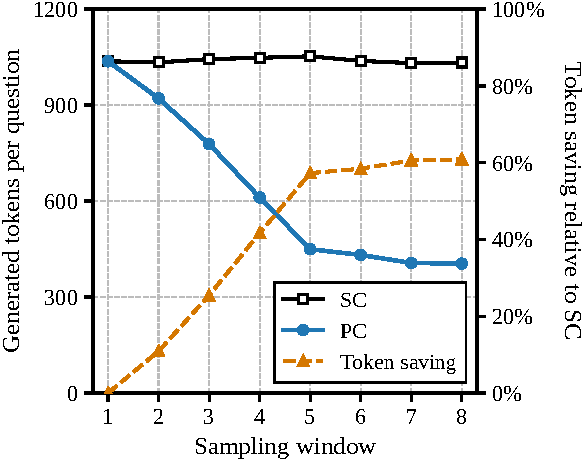
\includegraphics[width=\linewidth]{figs/window_tokens.pdf}
\caption{Tokens and savings by window.}
\label{fig:windows}
\end{minipage}
\end{figure}

Table~\ref{tab:prefix_levels} relates the extent of prefix reuse to the cost of subsequent generation. Windows are grouped by the nominal prefix level used, with level 0 including returns to the empty prefix. Prefix length counts one shared prefix, while generated tokens sum the four continuations per question. Across levels 1 to 4, mean prefix length increases from 39.4 to 177.5 tokens and generated tokens decrease from 859.3 to 256.7 per window. Relative to matched self-consistency windows, token savings rise from 14.3\% to 73.3\%, accompanied by generation-time reductions of 13.4\% to 73.6\%. Thus, higher prefix levels are associated with less remaining generation and larger measured savings.

Figure~\ref{fig:windows} shows how these savings develop over successive sampling windows, averaging over all 1,319 questions. Both methods start from the same unprefixed window. As shared prefixes extend, mean generated tokens under path-consistency decline from 1,036.8 in window 1 to 404.5 in window 8, whereas self-consistency remains near 1,040 tokens per window. The corresponding token saving reaches 60.9\% in the final window. By that point, 89.5\% of questions use a prefix, and mean prefix length across all questions reaches 158.6 tokens. Unlike the level-based groups in Table~\ref{tab:prefix_levels}, this window-level view includes questions at different prefix levels and those without a prefix.

Table~\ref{tab:prefix_case} illustrates the same progression through actual generated text. In this example, the shared prefix grows from 0 to 79 tokens over five windows. By the fourth window, it already contains the calculation of half of Haley's age, so later generation can continue from that intermediate result. By the fifth window, only the remaining subtraction and final answer need to be generated, using 26 tokens compared with 94 in the initial displayed trajectory. The expanding black prefix and shorter blue continuation make the source of the savings explicit. Together, the aggregate results and the example show how reusing intermediate reasoning reduces the generation required by later trajectories.

\begin{table}[t]
\centering\small
\caption{Progressive prefix reuse on a GSM8K example with Llama-3.1-8B-Instruct. Black text is the reused prefix and blue text is newly generated. One recorded trajectory is shown per window.}
\label{tab:prefix_case}
\begin{tabularx}{\linewidth}{@{}X@{}}
\toprule
\textbf{Question.} Geb is 10 less than half the age of Haley. If Haley is 26 years old, how old is Geb? \\
\midrule
\textbf{Window 1, prefix level 0\%} \hfill 0 prefix tokens; 94 generated tokens \\
{\color{blue}To find Geb's age, we need to follow these steps:  1. First, we find half of Haley's age. Haley is 26 years old, so half of her age would be 26 / 2 = 13.  2. Next, we need to subtract 10 from this half age to find Geb's age. So, 13 - 10 = 3.  Therefore, Geb is 3 years old.  $\boxed{3}$} \\
\midrule
\textbf{Window 2, prefix level 20\%} \hfill 17 prefix tokens; 104 generated tokens \\
To find Geb's age, we need to follow these steps:  1. First,\ {\color{blue} we need to find half of Haley's age. Haley is 26 years old, so half of 26 is 26 / 2 = 13.  2. Since Geb is 10 less than half the age of Haley, we need to subtract 10 from the half of Haley's age. So, Geb's age is 13 - 10.  3. Now, let's calculate 13 - 10 = 3.  Therefore, Geb is 3 years old.  $\boxed{3}$} \\
\midrule
\textbf{Window 3, prefix level 40\%} \hfill 34 prefix tokens; 75 generated tokens \\
To find Geb's age, we need to follow these steps:  1. First, we need to find half of Haley's age. Haley is 26 years old,\ {\color{blue} so half of her age would be 26 / 2 = 13.  2. Now that we have half of Haley's age, we need to subtract 10 from this number to find Geb's age.   3. So, Geb's age would be 13 - 10 = 3.  Therefore, Geb is $\boxed{3}$ years old.} \\
\midrule
\textbf{Window 4, prefix level 60\%} \hfill 52 prefix tokens; 56 generated tokens \\
To find Geb's age, we need to follow these steps:  1. First, we need to find half of Haley's age. Haley is 26 years old, so half of her age would be 26 / 2 = 13.  2.\ {\color{blue} Since Geb is 10 less than half the age of Haley, we need to subtract 10 from the half of Haley's age. So, Geb's age would be 13 - 10 = 3.  Therefore, Geb is $\boxed{3}$ years old.} \\
\midrule
\textbf{Window 5, prefix level 80\%} \hfill 79 prefix tokens; 26 generated tokens \\
To find Geb's age, we need to follow these steps:  1. First, we need to find half of Haley's age. Haley is 26 years old, so half of her age would be 26 / 2 = 13.  2. Since Geb is 10 less than half the age of Haley, we need to subtract 10 from the half of Haley's age.\ {\color{blue} So, 13 - 10 = 3.  Therefore, Geb is 3 years old.  $\boxed{3}$} \\
\bottomrule
\end{tabularx}
\end{table}


\subsection{Main results}
\label{sec:main_results}
\begin{table}[htbp]
\centering
\caption{Accuracy and token cost of long-chain reasoning with thinking enabled. PC uses the default $C=0.8$. Tokens are means per question; negative entries in Save indicate reductions relative to SC. MATH-500 accuracy is raw grading on 490 evaluated questions plus ten held-out engineering items counted as correct ($n=500$). Qwen/MATH-500 reports 199 evaluated questions and does not use this $n=500$ convention. DeepSeek GSM8K records are documented in Appendix~\ref{app:threshold}.}
\label{tab:main}
\setlength{\tabcolsep}{5pt}
\begin{tabular}{llcccccc}
\toprule
Model & Dataset & \multicolumn{3}{c}{Accuracy (\%)} & \multicolumn{3}{c}{Tokens (\# per problem)}\\
\cmidrule(lr){3-5}\cmidrule(lr){6-8}
 & & Pass@1 & SC & PC & SC & PC & Save (\%)\\
\midrule
DeepSeek-V4-Flash  & GSM8K & 96.74 & 96.82 & 96.82 & 12,514 & 8,230 & -34.2 \\
& MATH-500 & 86.60 & 88.00 & 87.60 & 41,166 & 26,968 & -34.5 \\
 & AIME 2024 & 93.33 & 96.67 & 96.67 & 288,230 & 213,162 & -26.0 \\
 & AIME 2025 & 86.67 & 100.00 & 100.00 & 351,230 & 260,523 & -25.8 \\
 & GPQA-D & 83.33 & 89.90 & 89.90 & 309,325 & 221,526 & -28.4 \\

\midrule
Qwen3-30B-A3B & GSM8K & 96.59 & 96.74 & 96.59 & 57,859 & 33,564 & -42.0 \\
& MATH-500 & 93.97 & 94.47 & 94.47 & 156,956 & 92,106 & -41.3 \\
 & AIME 2024 & 73.33 & 83.33 & 83.33 & 443,797 & 261,149 & -41.2 \\
 & AIME 2025 & 73.33 & 83.33 & 83.33 & 559,278 & 360,577 & -35.5 \\
 & GPQA-D & 61.76 & 62.94 & 62.35 & 234,446 & 152,079 & -35.1\\
\bottomrule
\end{tabular}
\end{table}

Table~\ref{tab:main} evaluates DeepSeek-V4-Flash and Qwen3-30B-A3B, both generating long reasoning chains with thinking enabled. Across the ten reported settings, path-consistency reduces generated tokens by 25.8\% to 42.0\%, averaging 34.4\% with equal weight assigned to each setting, while largely maintaining voting accuracy.

DeepSeek matches self-consistency's accuracy on GSM8K, both AIME benchmarks, and GPQA-D, and remains within 0.40 percentage points on MATH-500, with an average token saving of 29.8\%. Qwen achieves larger relative savings on every benchmark, averaging 39.0\%, with matching accuracy on MATH-500 and both AIME benchmarks and closely comparable accuracy on GSM8K and GPQA-D. Thus, the efficiency benefit appears across both models rather than being confined to a single setting.

Both models also retain gains over Pass@1 on the AIME benchmarks, showing that reduced generation cost need not eliminate the benefit of multiple sampled paths. Together with Section~\ref{sec:llama}, these results support prefix reuse for both shorter reasoning traces and long thinking chains as a way to reduce token cost while retaining the benefits of answer aggregation.

\subsection{Comparisons and composition}
\label{sec:composition}
Table~\ref{tab:composition} compares path-consistency with reasoning-sharing methods and evaluates its combination with early-stopping methods on Llama-3.1-8B-Instruct and GSM8K. Self-consistency with a reduced budget of $B=20$ provides an additional comparison at a similar token cost. The combinations retain the stopping and aggregation rules of adaptive-consistency and early-stopping self-consistency, so their additional savings are measured relative to each method without prefix reuse.

\begin{table}[htbp]
\centering\small
\caption{Method comparisons and early-stopping combinations on Llama-3.1-8B-Instruct/GSM8K. Tokens are means per question; negative entries in Save indicate reductions relative to SC with $B=32$. The maximum trajectory budget is 32 unless otherwise indicated. Indented rows add PC to the preceding method.}
\label{tab:composition}
\begin{tabular}{lrrr}
\toprule
Method & Accuracy (\%) & Tokens & Save (\%)\\
\midrule
Self-consistency & 92.12 & 8,316 & - \\
Self-consistency ($B=20$) & 91.28 & 5,214 & -37.3\% \\
PoLR ($L_p=128$) & 92.19 & 5,863 & -29.5\% \\
CPT (32 workers) & 92.80 & 8,411 & +1.1\% \\
Path-consistency & 91.74 & 5,039 & -39.4\% \\
\midrule
Adaptive-consistency ($\tau=0.95$) & 92.04 & 4,035 & -51.4\% \\
 \quad + Path-consistency & 92.27 & 3,003 & -63.9\% \\
Early-stopping self-consistency & 92.49 & 4,299 & -48.3\% \\
 \quad + Path-consistency & 92.27 & 3,501 & -57.9\% \\
\bottomrule
\end{tabular}
\end{table}

Path-consistency reduces generated tokens by 39.4\% relative to self-consistency while largely maintaining accuracy. Compared with simply reducing the trajectory budget to 20, it achieves higher accuracy with fewer tokens, supporting prefix reuse as an alternative to discarding sampling opportunities. Among the reasoning-sharing methods, path-consistency uses 14.1\% fewer tokens than PoLR, with closely comparable accuracy. CPT achieves the highest accuracy in this comparison but generates slightly more tokens than self-consistency. These results place path-consistency at a lower token cost rather than establishing uniform superiority across both accuracy and efficiency.

Prefix reuse also complements early stopping. Combined with adaptive-consistency, it reduces mean tokens from 4,035 to 3,003, an additional 25.6\% saving, while accuracy increases from 92.04\% to 92.27\%. Combined with early-stopping self-consistency, it reduces mean tokens from 4,299 to 3,501, an additional 18.6\% saving, while largely maintaining accuracy. Thus, path-consistency reduces generation cost both as a standalone reasoning-sharing method and in combination with early-stopping methods, providing further savings of 18.6\% to 25.6\% over the latter in this evaluation.

\subsection{Ablation studies}
\label{sec:ablations}
\paragraph{Contributions of prefix selection and recovery.}
Table~\ref{tab:selrec} examines local confidence selection and recovery on DeepSeek-V4-Flash/MATH-500 by replacing the selector with uniform selection, disabling recovery, or combining both changes. All configurations use the same 490 evaluated questions and shared self-consistency roots. Accuracy counts the ten held-out engineering items as correct ($n=500$). The remaining settings are fixed; implementation details are given in Appendix~\ref{app:ablation_design}.

\begin{table}[htbp]
\centering\small
\caption{Effects of prefix selection and recovery on DeepSeek-V4-Flash/MATH-500. Accuracy uses raw grading on 490 evaluated questions plus ten held-out engineering items counted as correct ($n=500$). $\Delta$ and Save denote the accuracy difference in percentage points and token reduction relative to SC. Tokens are means per evaluated question.}
\label{tab:selrec}
\begin{tabular}{lrrrr}
\toprule
Method & Accuracy (\%) & $\Delta$ (pp) & Tokens & Save (\%)\\
\midrule
SC & 88.00 & 0.00 & 41,166 & 0.0 \\
\midrule
PC (full) & 87.60 & $-0.40$ & 26,968 & 34.5 \\
\quad w/ uniform selection & 87.20 & $-0.80$ & 25,680 & 37.6 \\
\quad w/o recovery & 86.60 & $-1.40$ & 24,757 & 39.9 \\
\quad w/ uniform selection, w/o recovery & 86.60 & $-1.40$ & 25,405 & 38.3 \\
\bottomrule
\end{tabular}
\end{table}

The full configuration achieves the highest accuracy among the path-consistency variants at 87.60\%, while saving 34.5\% of generated tokens. Uniform selection lowers accuracy to 87.20\%, and disabling recovery lowers it to 86.60\% under either selector. The variants save more tokens, but at the cost of lower accuracy. These results support retaining both components when accuracy preservation is prioritized, with recovery showing the larger observed contribution in this setting.

\paragraph{Sensitivity to the agreement threshold.}
Table~\ref{tab:threshold} examines the trade-off between accuracy and token savings across agreement thresholds on DeepSeek-V4-Flash/GSM8K, with $C=1$ corresponding to self-consistency. The default $C=0.8$ preserves its 96.82\% accuracy while reducing generated tokens by 34.2\%. Lowering $C$ to 0.7 and 0 increases savings to 40.8\% and 43.5\%, respectively, with small accuracy decreases of 0.08 and 0.23 percentage points.

\begin{table}[htbp]
\centering
\caption{Accuracy and token cost across agreement thresholds on DeepSeek-V4-Flash/GSM8K. Tokens are means per question. $\Delta$ and Save report changes relative to SC ($C=1$), with negative Save values indicating token reductions.}
\label{tab:threshold}
\begin{tabular}{lcccc}
\toprule
Threshold ($C$) & Accuracy (\%) & $\Delta$ (pp) & Tokens (\# per problem) & Save (\%)\\
\midrule
1.0 (Self-consistency) & 96.82 & - & 12,514 & - \\
0.8  & 96.82 & 0.00 & 8,230 & -34.2\\
0.7  & 96.74 & -0.08 & 7,399 & -40.8\\
0  & 96.59 & -0.23  & 7,070 & -43.5\\
\bottomrule
\end{tabular}
\end{table}

A lower threshold permits prefix reuse under weaker answer agreement, whereas a higher threshold requires stronger agreement and makes reuse more conservative. The threshold therefore offers a direct way to express user priorities. Lower values favor more efficient generation through greater token savings, while higher values favor accuracy preservation.
